\section{Квантовая яма CdTe--HgTe--CdTe в модели сильной связи}
В этом разделе будет построена модель сильной связи, эквивалентная $k\cdot p$ гамильтониану
\eqref{kane_ham}. Численно диагонализуя её, можно независимо получить уровни размерного 
квантования.
\subsection{Модель однородного полупроводника}
Модель представляет из себя 
кубическую решётку из атомов, на каждом из которых ``сидят'' состояния
с $p_x$, $p_y$, $p_z$ и $s$--орбиталями и двумя 
возможными проекцими спина.

Для написания
спин--орбитального гамильтониана $p$--зоны необходимо перейти к состояниям с определённым
полным моментом. Эти состояния выражаются через $p_x$, $p_y$, $p_z$ орбитали через
коэффициенты Клебша--Гордана (см. приложение~\ref{app:tb}).

Спин--орбитальное взаимодействие приводит к расщеплению состояний с моментами $\frac32$ и
$\frac12$.
Состояниями с полным моментом $\frac{1}{2}$ 
можно пренебречь, если спин--орбитальное взаимодейтвие велико. Таким образом, в каждом
узле решётки остаётся пара $s$--орбиталей, формирующая валентную зону, и четыре состояния
с полным моментом $\frac{3}{2}$. Матричные элементы перекрытия между состояниями на соседних
узлах выражаются через перекрытия $s$ и $p$ орбиталей с использованием выражений 
\eqref{transform1}. 

Определим матричные элементы $t_\parallel$ и $t_\perp$ для перекрытия соседних $p$--орбиталей,
расположенных соответственно <<вдоль>> и <<поперёк>>, $\frac{-iP}{2}$ для перекрытия
$s$ и $p$--орбитали и $-\frac{1}{2m_s}$ --- для $s$--орбиталей. Через них полный гамильтониан
сильной связи записывается в импульсном представлении в виде огромной матрицы $6\times6$. 

\begin{equation}
    \label{hfull}
    H_{\mathrm{full}} = \begin{pmatrix}
                            H_c & T \\
                            T^\dagger & H_v
                        \end{pmatrix},
\end{equation}
Матрицы $H_c$, $T$, $H_v$ определены формулами \eqref{H_conduction}--\eqref{H_valence}, см.
стр.~\pageref{H_conduction}.
Этот гамильтониан можноразложить по малым $p$,
в результате чего получится гамильтониан Латтинжера:
\begin{equation}
    H_v = \frac{\hbar^2}{2ma^2}\left\{-\left(\gamma_1 + \frac{5}{2}\gamma_2\right) k^2 + 
        2\gamma_2(k_x^2J_x^2 + k_y^2J_y^2 + k_z^2J_z^2) + 
        4\gamma_3(k_x k_y J_x J_y + k_x k_z J_x J_z + k_y k_z J_y J_z) \right\}
\end{equation}
Здесь $J_i$ --- операторы момента для спина $\frac{3}{2}$, $a$ --- постоянная решётки,
$m$ --- масса электрона,
\begin{equation}
    \begin{gathered}
        \frac{\hbar^2}{2ma^2}\gamma_1 = \frac13 t_\parallel\\
        \frac{\hbar^2}{2ma^2}\gamma_2 = \frac16(t_\parallel - t_\perp)\\
        \gamma_3 = 0\\
    \end{gathered}
\end{equation}
Разложение $H_c$ и $T$ тривиально.
Всё это вместе воспроизводит модель Кейна, которую обычно получают в $k \cdot p$ приближении.

Коэффициенты перескока в сильной связи можно зафиксировать требованием, чтобы при малых $p$ 
воспроизводился $k\cdot p$ гамильтониан с значениями параметров, известных из эксперимента
\cite{Novik2005}. 

\subsection{Модель квантовой ямы}
Квантовая яма представляет из себя последовательно расположенные слои CdTe, HgTe и CdTe.
Это можно непосредственно реализовать как модель сильной связи с двумя типами узлов, которую
затем несложно диагонализовать численно. Спектр этой модели состоит из густо расположенных
двумерных зон, соответствующих объёмным состояниям CdTe, и двумерных зон размерного квантования
HgTe, расположенных в запрещённой зоне CdTe.

Для двух уровней размерного квантования можно написать эффективный гамильтониан,
учитывающий только их. Оказывается, что этот гамильтониан при малых $k_x,k_y$ превращается
в две копии 
\eqref{BHZ}, переходящие друг в друга при обращении времени. $\xi$ из гамильтониана \eqref{BHZ} --- это расстояние между уровнями размерного
квантования при $k_x, k_y$. Таким образом, в тот момент, когда два уровня размерного 
квантования пересекаются, эффективный гамильтониан для этих уровней становится 
гамильтонианом топологического изолятора. Согласно \cite{Bernevig2006}, это происходит
при толщине ямы, равной $6.4$ nm. У меня получилось, что критическая толщина равна
$\approx 7.5$ nm.

\begin{figure}[h]
    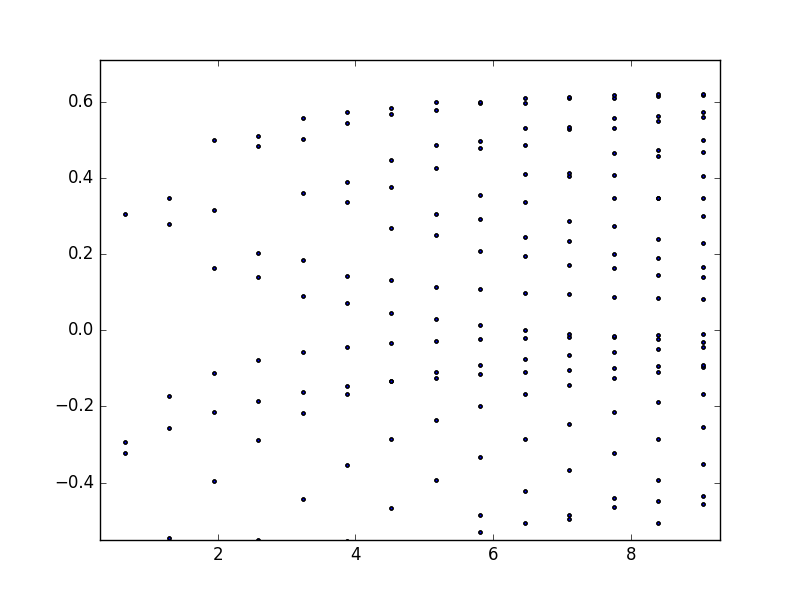
\includegraphics[width=0.8\linewidth]{dim_quant_levels.png}
    \caption{
            На графике изображены уровни размерного квантования, полученные 
            численной диагонализацией, для $k_x, k_y = 0$
            в зависимости от толщины слоя HgTe, nm. Видно, что два уровня размерного
            пересекаютcя при $d \approx 7.5$.
            }
\end{figure}
